% SNAS 2026 double-blind short-paper submission candidate.
% Compile with XeLaTeX so the document uses the installed Times New Roman font.
\documentclass[12pt,letterpaper,twoside]{article}

\usepackage[margin=1in]{geometry}
\usepackage{fontspec}
\setmainfont{Times New Roman}
\usepackage{setspace}
\doublespacing
\usepackage{booktabs}
\usepackage{graphicx}
\usepackage{fancyhdr}
\usepackage{titlesec}
\usepackage{xurl}
\urlstyle{same}
\usepackage[hidelinks]{hyperref}
\hypersetup{
  pdftitle={Beyond Stable Answers: Auditing Explanation Faithfulness in a Construction-Safety Vision-Language Pipeline},
  pdfauthor={},
  pdfsubject={Double-blind submission candidate for the 5th SNAS Interdisciplinary Research Conference},
  pdfkeywords={explainable artificial intelligence, vision-language models, construction safety, explanation faithfulness}
}

\setlength{\parindent}{0.5in}
\setlength{\parskip}{0pt}
\setlength{\emergencystretch}{3em}
\setlength{\textfloatsep}{10pt plus 2pt minus 2pt}
\setlength{\floatsep}{8pt plus 2pt minus 2pt}
\raggedbottom

\titleformat{\section}
  {\normalfont\bfseries\centering}
  {\thesection.}{0.5em}{}
\titlespacing*{\section}{0pt}{10pt}{5pt}
\titleformat{\subsection}
  {\normalfont\bfseries}
  {\thesubsection.}{0.5em}{}
\titlespacing*{\subsection}{0pt}{7pt}{2pt}

\pagestyle{fancy}
\fancyhf{}
\fancyhead[LE,LO]{\textit{Beyond Stable Answers}}
\fancyhead[RE,RO]{\thepage}
\renewcommand{\headrulewidth}{0.4pt}
\setlength{\headheight}{15pt}

\newenvironment{apareferences}
  {\begin{list}{}{%
    \setlength{\leftmargin}{0.5in}%
    \setlength{\itemindent}{-0.5in}%
    \setlength{\itemsep}{0pt}%
    \setlength{\parsep}{0pt}%
    \setlength{\topsep}{0pt}}}
  {\end{list}}

\begin{document}

\begin{center}
\textbf{Beyond Stable Answers: Auditing Explanation Faithfulness in a Construction-Safety Vision-Language Pipeline}
\end{center}

\begin{center}
\textbf{Abstract}
\end{center}

Vision-language models (VLMs) may support construction-safety review, but answer accuracy alone does not show whether a judgment depends on relevant visual evidence. This feasibility and construct-validity study adapts a six-dimensional explainable artificial intelligence evaluation framework to a VLM-grounded construction-safety pipeline. Florence-2-base-ft grounded workers and rule-relevant objects in 163 held-out ConstructionSite 10k images; deterministic person-relative geometry then produced the safety verdict. The pipeline was not native free-form visual question answering. Explanations were audited through semantic region ranking, safety-object masking, worker-loss correction, and paired targeted-versus-control interventions. The primary control placed five seeded black rectangles per image, each exactly matching the targeted object's clipped width and height. Area ranking selected the worker instead of the safety object in 50.3\% of usable cases; rule-aware ranking reduced this to 0.6\%. Among 158 images with a valid target, targeted masking changed 39.2\% of verdicts versus 9.2\% under matched-random masking, a paired difference of 30.0 percentage points (95\% CI [22.3, 37.7]). Targeted normalized centroid drift was 0.196 versus 0.031 for the control, a difference of 0.166 (95\% CI [0.140, 0.193], Holm-adjusted \textit{p} < .001, rank-biserial \textit{r} = .892). In secondary stable-answer analyses, intersection-over-union flagged 22.1\% of cases while size-invariant centroid relocation flagged 12.3\%; the discrepancy was largest for small boxes. These results show that output stability, evidence movement, and evidence availability must be measured separately. The low-sensitivity pipeline remains a research testbed requiring human oversight, not an autonomous safety system.

\noindent\textit{Keywords:} explainable artificial intelligence; vision-language models; construction safety; explanation faithfulness; robustness; trustworthy AI

\section{Introduction}

Construction and extraction occupations recorded 1,032 fatal work injuries in the United States in 2024, a rate of 12.6 per 100,000 full-time-equivalent workers (U.S. Bureau of Labor Statistics [BLS], 2026). Human inspection remains essential, while image-based systems may help trained personnel review site evidence and prioritize follow-up. Recent VLM research has expanded construction-image analysis from object detection toward contextual hazard classification, captioning, and rule-based questioning (Adil et al., 2025, 2026; Chen \& Zou, 2026; Kim et al., 2025; Li et al., 2026).

Capability does not establish trustworthy use. A system may return a stable verdict while its grounding moves to an unrelated object, and a plausible visual rationale need not reflect evidence on which the output depends (Jain \& Wallace, 2019; Li et al., 2025). Conversely, an answer may change because an intervention breaks an upstream detector rather than removes the intended safety cue. These distinctions matter in safety review because output stability, evidence movement, and evidence availability create different failure modes.

This study adapts the descriptive accuracy, sparsity, stability, efficiency, robustness, and completeness dimensions of an XAI evaluation framework developed for network-intrusion detection (Arreche et al., 2024; Arreche \& Abdallah, 2025). The framework transfers conceptually, but visual grounding adds region-ranking choices, box-size effects, masking artifacts, and detector fallback paths. We ask: (1) whether occluding a rule-relevant object changes the verdict or grounding more than an exactly same-size random-location control; (2) how semantic region ranking changes the construct being tested; and (3) whether IoU overstates explanation movement for small boxes. The contribution is a reproducible construct-validity audit, not evidence of deployment readiness or human trust calibration.

\section{Related Work}

ConstructionSite 10k provides 10,013 images with captions, safety-rule questions, rationales, and grounding annotations (Chen \& Zou, 2026). Other studies have evaluated general-purpose VLMs for construction hazards, adapted models for context-aware assessment and fall-hazard captioning, and combined detectors with smaller VLMs (Adil et al., 2025, 2026; Kim et al., 2025; Li et al., 2026). This literature establishes emerging task capability but leaves a complementary question: whether the evidence associated with a safety judgment remains relevant and stable under intervention.

Faithfulness concerns whether an explanation reflects the basis for an output or the process that produced it (Phillips et al., 2021). Prior work cautions that visually persuasive attention or rationale outputs should not automatically be treated as explanations (Jain \& Wallace, 2019), and recent vision research shows that perturbation metrics can fail to distinguish advanced explanations from random attribution when their assumptions are not validated (Wu et al., 2024). Explainable VQA research likewise notes that correct answers can coexist with irrelevant visual focus (Li et al., 2025).

The NIST AI Risk Management Framework emphasizes context, construct validation, documentation, and defined human oversight (National Institute of Standards and Technology [NIST], 2023). NIOSH guidance similarly treats workplace AI as a source of both potential benefit and worker risk (Howard \& Schulte, 2024). Accordingly, the present study evaluates technical intervention behavior. It does not claim that an explanation is meaningful to a safety professional, improves calibrated reliance, or reduces injuries.

\section{Method}

\subsection{Data, Model, and Decision Pipeline}

A fixed, seed-42 sample was drawn from the 3,004-image test split of ConstructionSite 10k. Priority labeling and class-balanced sampling yielded 50 compliant scenes, 50 PPE violations, 50 fall hazards, and all 13 available struck-by-risk cases, for 163 unique images. The struck-by subgroup was retained for coverage but treated as exploratory because \textit{n} < 30. The dataset revision was ca3d9b8 and its CC BY-NC 4.0 license governed use.

The model was \textit{microsoft/Florence-2-base-ft}, revision f6c1a25, an approximately 0.23-billion-parameter sequence-to-sequence model supporting prompted detection and grounding (Xiao et al., 2024). Beam decoding used three beams. In this implementation Florence-2 did not expose native free-form VQA. It grounded a worker and a rule-relevant object---hard hat, harness, guardrail, or excavator---and deterministic person-relative geometry converted those boxes into a compliant, violation, or hazard verdict. The object box associated with the assigned rule served as the primary visual explanation.

\subsection{Interventions and Outcomes}

The frozen baseline ranked candidate regions by pixel area. Because this frequently promoted a worker body over small PPE, a rule-aware policy ranked the queried safety-object class first and used area only within semantic tiers. Top-region masking was rerun under this policy. A verdict flip that coincided with loss of the only baseline worker detection was labeled a worker-loss failure; corrected flip rates excluded those failures.

The primary experiment used the first baseline safety-object box for each of 158 images with a valid target. Targeted intervention replaced that exact clipped rectangle with black pixels. For each image, five control masks used the same clipped width and height but seeded random locations (42--46). Each seed sampled up to 200 locations seeking mask-target IoU at or below 0.05; if geometry made that impossible, the lowest-overlap candidate was retained. Thus area, color, and inference count were controlled, while location relative to the safety object varied. Random outcomes were averaged within image before paired analysis. A low-overlap sensitivity analysis retained only control placements with mask-target IoU at or below 0.05.

The outcomes were verdict change; worker-loss-corrected verdict change; movement of the object box measured by centroid displacement divided by image diagonal; and explanation disappearance when a baseline object had no perturbed counterpart. A secondary multi-operator severity sweep examined stable-answer rows using IoU below 0.3 and centroid drift above 0.2. Baseline object-area tertiles tested whether IoU failure varied with box size.

\subsection{Statistical and Reproducibility Protocol}

The image was the analysis unit. Rates and means used 10,000 fixed-seed percentile-bootstrap resamples, and paired differences resampled image-level differences. Two-sided Wilcoxon signed-rank tests compared targeted with within-image mean control outcomes; Holm adjustment covered the two primary comparisons. Matched-pairs rank-biserial correlation quantified effect direction and magnitude. Ninety-five percent intervals are reported without making confirmatory class-level claims for the 13-image struck-by subgroup.

Experiments ran with Python 3.10.11, PyTorch 2.12.1+cu130, Transformers 4.49.0, and one NVIDIA RTX 3070. The paper-owned intervention file contains 948 unique rows: 158 targeted and 790 control rows. Automated checks verified exact mask-area equality, row-key uniqueness, consistency with the validated targeted run, and deterministic statistical output. Source inputs, software versions, and SHA-256 hashes are recorded in an artifact manifest. The source test suite passed 179 tests; seven paper-analysis tests also passed.

\section{Results}

\subsection{Task Capability and Region Validity}

The decision pipeline's violation sensitivity was 31.0\% (95\% CI [23.0, 39.8]) and compliant specificity was 66.0\% (95\% CI [52.0, 78.0]). These values are inadequate for field deployment but sufficient to expose explanation-evaluation failure modes in a working pipeline.

Among 159 images with model-provided candidate regions, area ranking selected a worker as top-1 in 50.3\% (95\% CI [42.8, 57.9]). Rule-aware ranking reduced worker top-1 selection to 0.6\% (95\% CI [0.0, 1.9]). The corrected rule-aware top-region ablation changed 37.4\% of verdicts (95\% CI [30.1, 44.8]). Semantic ranking therefore changed the intervention from a test of dependence on the largest object to a test of dependence on rule-relevant evidence.

\subsection{Targeted Versus Matched-Random Occlusion}

Table~\ref{tab:primary-results} and Figure~\ref{fig:primary-results} summarize the primary experiment. Targeted masks changed 39.2\% of verdicts, compared with 9.2\% under the per-image mean of five same-size random masks. The paired difference was 30.0 percentage points (95\% CI [22.3, 37.7], Holm-adjusted \textit{p} < .001, rank-biserial \textit{r} = .888). Worker-loss correction changed the estimates only modestly, to 38.0\% and 8.7\%, respectively.

\begin{table}[t]
\centering
\caption{Primary Intervention Results with Bootstrap 95\% Confidence Intervals}
\label{tab:primary-results}
\begin{tabular}{@{}lcc@{}}
\toprule
Outcome & Targeted & Matched random \\
\midrule
Answer change & 39.2\% [31.6, 46.8] & 9.2\% [5.7, 13.2] \\
Corrected answer change & 38.0\% [30.4, 45.6] & 8.7\% [5.3, 12.4] \\
Centroid drift & 0.196 [0.170, 0.222] & 0.031 [0.021, 0.043] \\
Disappearance & 5.1\% [1.9, 8.9] & 3.7\% [1.1, 6.7] \\
\bottomrule
\end{tabular}
\begin{minipage}{0.94\linewidth}
\vspace{2pt}\footnotesize Note. Random estimates average five same-size placements per image. Targeted minus random answer change = 30.0 percentage points (95\% CI [22.3, 37.7]); centroid-drift difference = 0.166 (95\% CI [0.140, 0.193], Wilcoxon \textit{p} < .001, rank-biserial \textit{r} = 0.892, \textit{n} = 149).
\end{minipage}
\end{table}


Targeted centroid drift averaged 0.196, compared with 0.031 under matched-random occlusion. Among 149 complete pairs, the difference was 0.166 (95\% CI [0.140, 0.193], Holm-adjusted \textit{p} < .001, rank-biserial \textit{r} = .892). Disappearance was less clearly separated: 5.1\% targeted versus 3.7\% control. Overall, 88.2\% of random placements met the IoU-at-most-0.05 goal. In the conservative low-overlap sensitivity subset (140 images), random-mask verdict change fell to 8.0\% (95\% CI [4.6, 11.9]), preserving the interpretation that targeted location, not mask area alone, drove most changes.

\begin{figure}[t]
\centering
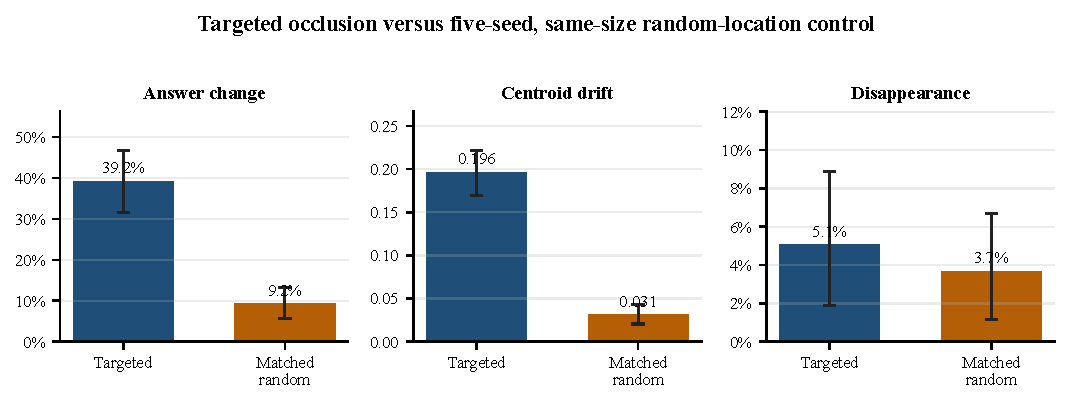
\includegraphics[width=\linewidth]{figures/targeted_vs_matched_random.pdf}
\caption{Primary outcomes. Error bars are bootstrap 95\% confidence intervals; matched-random values are per-image averages over five same-size placements.}
\label{fig:primary-results}
\end{figure}

\subsection{Stable Answers, Size Bias, and Failure Accounting}

Across non-targeted conditions in the secondary sweep, the per-image mean stable-answer IoU-failure rate was 22.1\% (95\% CI [19.2, 25.1]), while centroid relocation above 0.2 occurred in 12.3\% (95\% CI [10.1, 14.5]). IoU failure decreased from 30.5\% for small baseline boxes to 23.9\% for medium and 12.0\% for large boxes. The corresponding centroid rates were 17.4\%, 11.7\%, and 7.6\%. IoU therefore detected genuine movement but also amplified small-coordinate changes for small boxes.

Disappearance and worker loss required separate accounting. A missing post-intervention box cannot be represented by a conventional mean IoU if missing rows are silently dropped. Likewise, a changed verdict following worker-detector failure does not show dependence on the intended safety object. Recording both states prevented unavailable evidence and pipeline breakage from being mislabeled as ordinary explanation drift.

\section{Discussion}

The matched experiment supports a narrow claim: this pipeline was more sensitive to removal of the grounded safety object than to removal of an equally large region elsewhere. It does not prove that every grounding box was semantically correct or that the model's internal reasoning was recovered. That distinction is central to construct validity. Targeted-minus-control effects provide evidence of location-specific dependence, while semantic ranking determines which location is tested.

The study also shows why a stable verdict is an incomplete robustness result. Evidence may move while the verdict remains fixed, disappear entirely, or be replaced after a detector fallback. Reporting only answer survival would hide those cases. At the same time, reporting IoU alone would overstate movement for small boxes. A minimum audit should therefore report verdict change, a size-invariant movement measure, disappearance, upstream detector state, and an area-matched location control.

For practice, the appropriate framing is decision support with documented abstention and human review. A reviewer should be able to see the cited region, know when it is missing or unstable, and retain authority over the safety decision. Human-centered studies are still needed to test whether such disclosures improve calibrated reliance, workload, or decision quality (Naiseh et al., 2023). These controls align with risk-management guidance to document system limits, evaluate constructs in context, and define human oversight (NIST, 2023).

\section{Limitations and Ethics}

The study uses one compact model, one dataset, and one 163-image seeded sample. Only 13 struck-by cases were available, so subgroup inference is underpowered. The verdict is deterministic geometry over VLM grounding rather than native VQA, and the low sensitivity and specificity preclude deployment. Black rectangles are out-of-distribution artifacts, although exact area matching, five placements, overlap auditing, and worker-loss correction reduce alternative explanations. The secondary size-bias analysis uses a heterogeneous perturbation sweep and should be interpreted as metric validation rather than a new model-performance estimate. No external safety professional annotated the model's generated boxes for this study.

No human-subject study was conducted. The work does not establish trust, fairness, workload benefit, or injury reduction. Construction imagery may create privacy, surveillance, and labor-governance risks. The pipeline does not infer identity, intent, competence, or blame, and the dataset cannot support demographic fairness claims. Any future field study should use data minimization, notice, access controls, professional review, appeal procedures, and a prohibition on autonomous disciplinary action.

\section{Conclusion}

Answer stability did not guarantee stable or available visual evidence. Rule-aware ranking corrected region selection, and same-size random controls showed greater verdict change and explanation movement at targeted object locations than elsewhere. IoU overstated movement for small boxes. Trustworthy evaluation should separate output change, evidence movement, evidence availability, and upstream failure. This system is a research testbed, not an autonomous safety inspector.

\label{bodyend}
\clearpage
\section*{References}

\begin{apareferences}
\item Adil, M., Ahmed, M., Aqib, M., Gonzalez, V. A., Lee, G., \& Mei, Q. (2026). Integration of object detection and small VLMs for construction safety hazard identification. \textit{arXiv}. \url{https://arxiv.org/abs/2604.05210}

\item Adil, M., Lee, G., Gonzalez, V. A., \& Mei, Q. (2025). Using vision language models for safety hazard identification in construction. \textit{arXiv}. \url{https://arxiv.org/abs/2504.09083}

\item Arreche, O., \& Abdallah, M. (2025). A comparative analysis of DNN-based white-box explainable AI methods in network security. \textit{EURASIP Journal on Information Security, 2025}, Article 16. \url{https://doi.org/10.1186/s13635-025-00201-x}

\item Arreche, O., Guntur, T. R., Roberts, J. W., \& Abdallah, M. (2024). E-XAI: Evaluating black-box explainable AI frameworks for network intrusion detection. \textit{IEEE Access, 12}, 23954--23988. \url{https://doi.org/10.1109/ACCESS.2024.3365140}

\item Chen, X., \& Zou, Z. (2026). Are large pre-trained vision language models effective construction safety inspectors? \textit{Data-Centric Engineering, 7}, e11. \url{https://doi.org/10.1017/dce.2026.10044}

\item Howard, J., \& Schulte, P. A. (2024, September 9). Exploring approaches to keep an AI-enabled workplace safe for workers. \textit{National Institute for Occupational Safety and Health}. \url{https://www.cdc.gov/niosh/bulletin/2024/ai-risk-management.html}

\item Jain, S., \& Wallace, B. C. (2019). Attention is not explanation. In \textit{Proceedings of NAACL-HLT 2019} (pp. 3543--3556). \url{https://doi.org/10.18653/v1/N19-1357}

\item Kim, T., Kim, S., Chern, W.-C., Park, S., Kim, D., \& Kim, H. (2025). Optimizing large vision-language models for context-aware construction safety assessment. \textit{Automation in Construction, 180}, 106510. \url{https://doi.org/10.1016/j.autcon.2025.106510}

\item Li, K., Vosselman, G., \& Yang, M. Y. (2025). Multimodal rationales for explainable visual question answering. In \textit{Proceedings of the IEEE/CVF Conference on Computer Vision and Pattern Recognition Workshops} (pp. 191--201). \url{https://openaccess.thecvf.com/content/CVPR2025W/MULA2025/html/Li_Multimodal_Rationales_for_Explainable_Visual_Question_Answering_CVPRW_2025_paper.html}

\item Li, Y., Xu, F., Zhang, Z., Mei, X., \& Huang, H. (2026). Construction site fall hazard identification and automated captioning using adapted vision-language models. \textit{Automation in Construction, 183}, 106790. \url{https://doi.org/10.1016/j.autcon.2026.106790}

\item Naiseh, M., Al-Thani, D., Jiang, N., \& Ali, R. (2023). How the different explanation classes impact trust calibration: The case of clinical decision support systems. \textit{International Journal of Human-Computer Studies, 169}, 102941. \url{https://doi.org/10.1016/j.ijhcs.2022.102941}

\item National Institute of Standards and Technology. (2023). \textit{Artificial Intelligence Risk Management Framework (AI RMF 1.0)}. \url{https://doi.org/10.6028/NIST.AI.100-1}

\item Phillips, P. J., Hahn, C. A., Fontana, P. C., Yates, A. N., Greene, K., Broniatowski, D. A., \& Przybocki, M. A. (2021). \textit{Four principles of explainable artificial intelligence} (NISTIR 8312). National Institute of Standards and Technology. \url{https://doi.org/10.6028/NIST.IR.8312}

\item U.S. Bureau of Labor Statistics. (2026). \textit{Number and rate of fatal work injuries, civilian workers, by major occupational group, 2024}. \url{https://www.bls.gov/charts/census-of-fatal-occupational-injuries/number-and-rate-of-fatal-work-injuries-by-occupation.htm}

\item Wu, J., Kang, W., Tang, H., Hong, Y., \& Yan, Y. (2024). On the faithfulness of Vision Transformer explanations. In \textit{Proceedings of the IEEE/CVF Conference on Computer Vision and Pattern Recognition} (pp. 10936--10945). \url{https://openaccess.thecvf.com/content/CVPR2024/html/Wu_On_the_Faithfulness_of_Vision_Transformer_Explanations_CVPR_2024_paper.html}

\item Xiao, B., Wu, H., Xu, W., Dai, X., Hu, H., Lu, Y., Zeng, M., Liu, C., \& Yuan, L. (2024). Florence-2: Advancing a unified representation for a variety of vision tasks. In \textit{Proceedings of the IEEE/CVF Conference on Computer Vision and Pattern Recognition} (pp. 4818--4829). \url{https://openaccess.thecvf.com/content/CVPR2024/html/Xiao_Florence-2_Advancing_a_Unified_Representation_for_a_Variety_of_Vision_CVPR_2024_paper.html}
\end{apareferences}

\end{document}
